\documentclass[../main.tex]{subfiles}
\begin{document}

\chapter{Energilagring } \label{Chap:Energilagring}

\section{Sammenligning mellem teoretiske og reelle værdier}
testtest

\section{Test}
Krav 7 i kravspecifikationen siger at Spændingen V3 skal være indenfor 5v +/- 0.5 volt ved strømme større end 20 mA. Dette opfyldes 

\begin{figure}[H]
      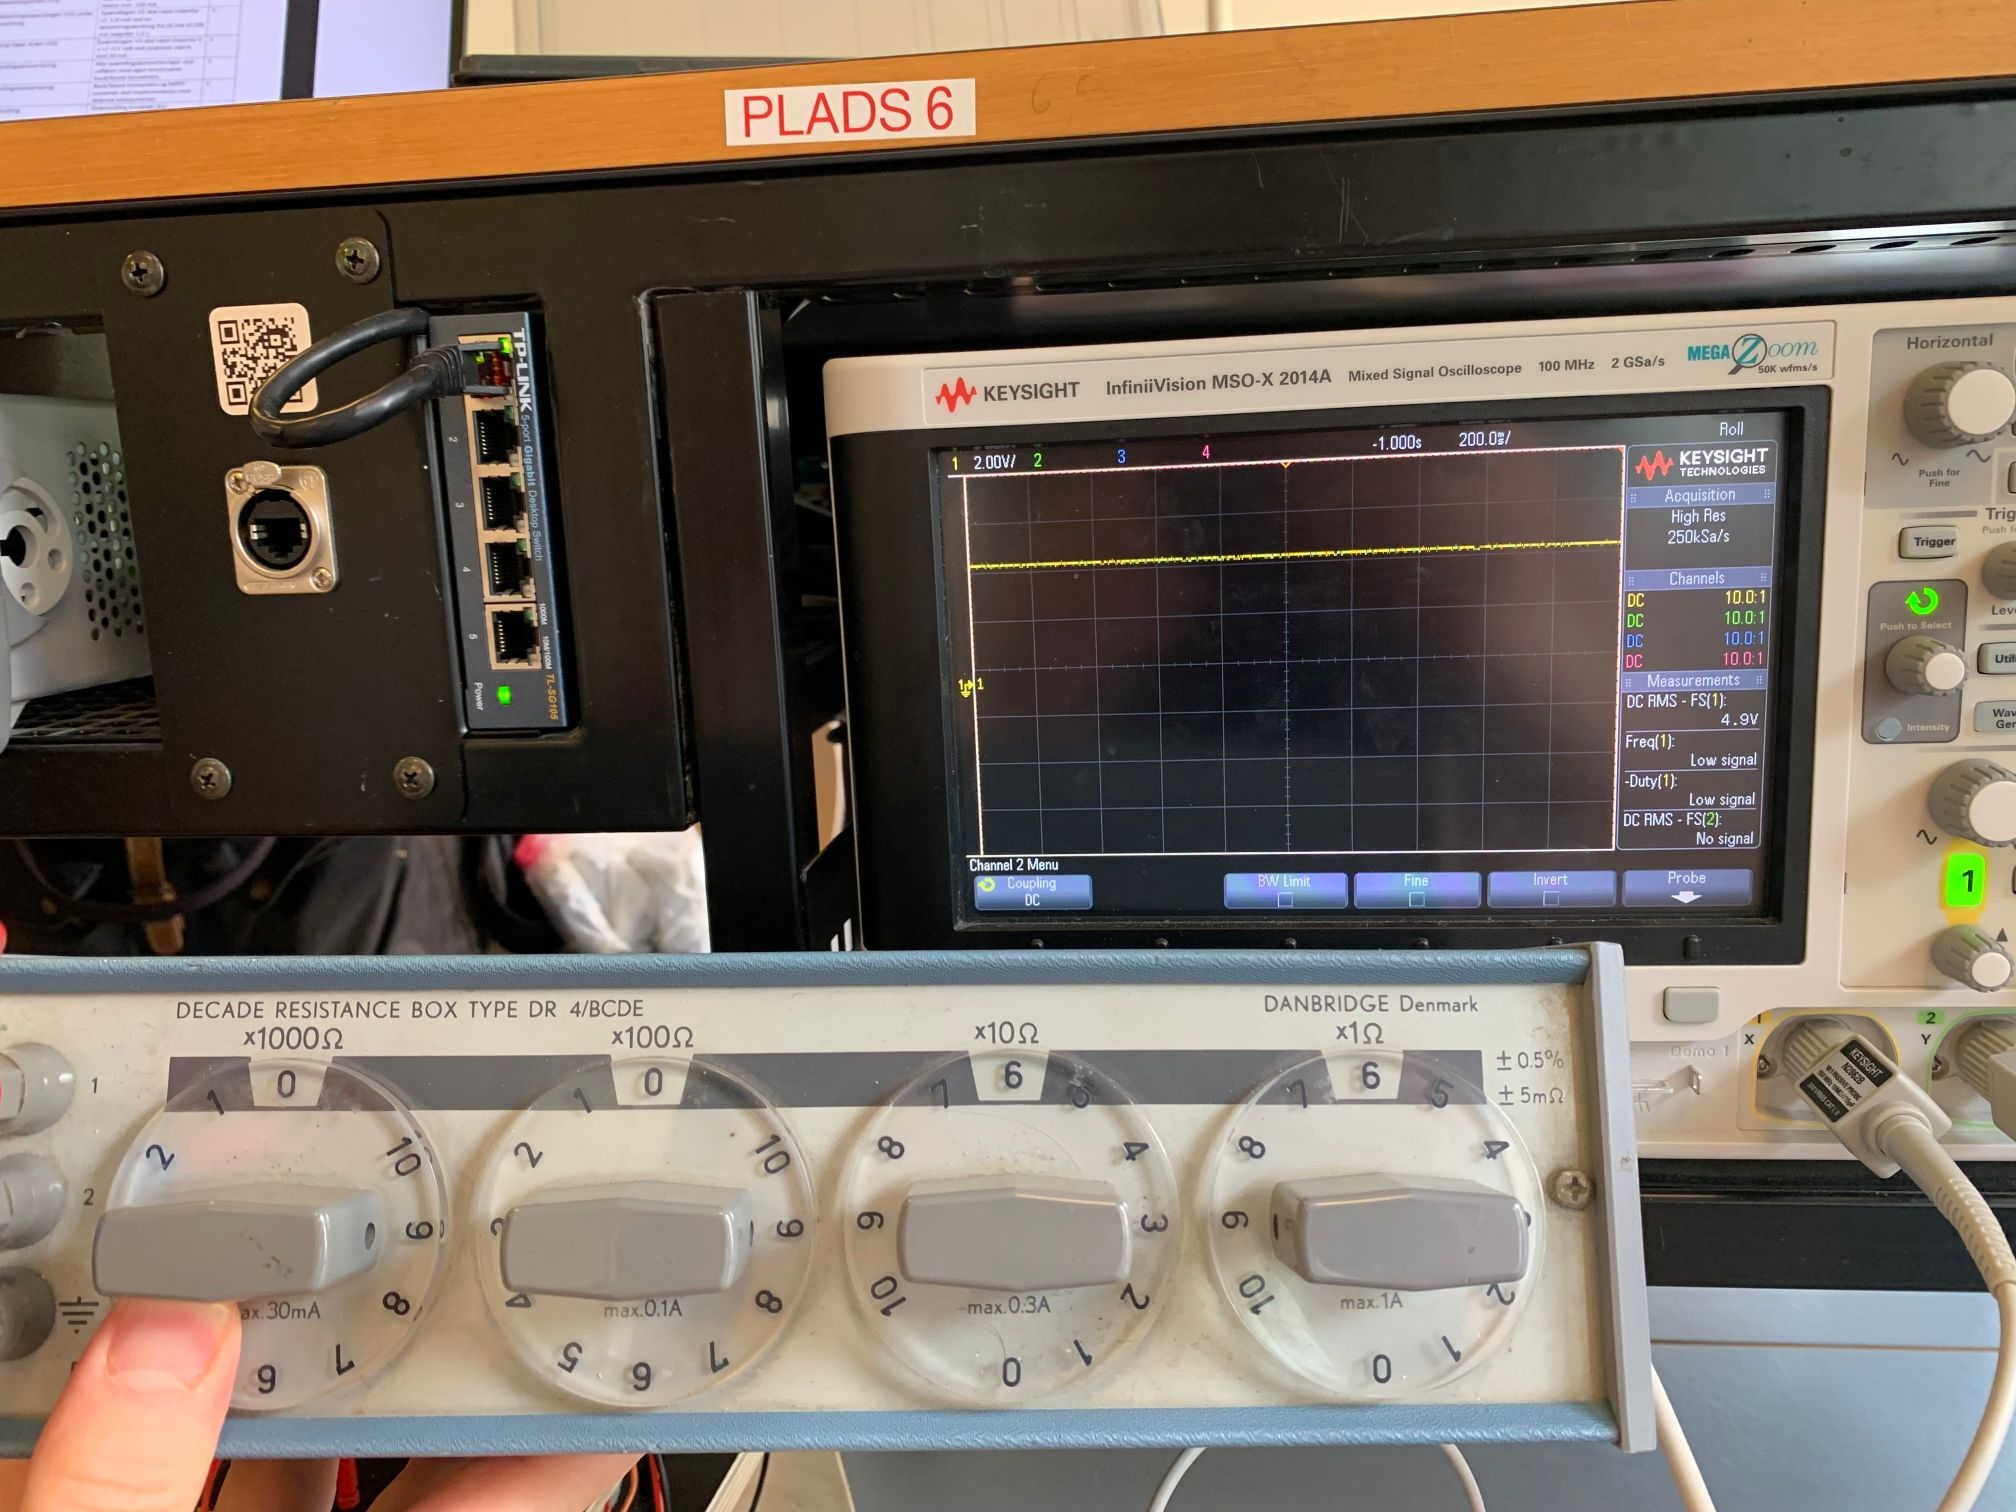
\includegraphics[width=\textwidth]{Dokumentation/Pictures/Krav7.jpg}
     \caption{Krav 7 Opfyldt}
     \label{fig: Krav 7 Opfyldt}
     \end{figure}


\end{document}

